\chapter{Binomial Bernoulli Distribution}
\textbf{Question:} Estimate the probability of the states of consecutive seven days ('Rain', 'Dry', 'Rain', 'Dry', 'Rain', 'Dry', 'Rain', 'Rain', 'Dry', 'Dry') using Markov Model.

\begin{figure}[H]
   \centering
   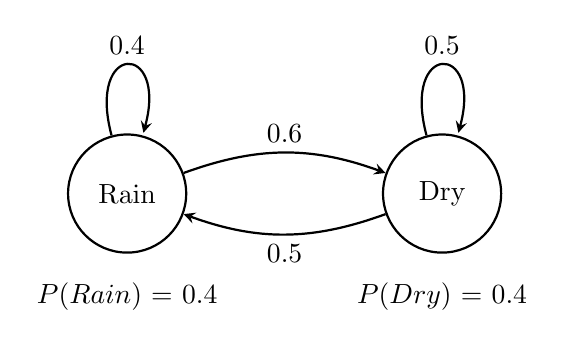
\begin{tikzpicture}[->, >=stealth, node distance=4cm, thick, main/.style = {draw, circle, minimum size=1.5cm}]
      \node[main] (Rain) {Rain};
      \node[main, right of=Rain] (Dry) {Dry};
   
      \path
         (Rain) edge[bend left=20] node[above] {0.6} (Dry)
         (Dry) edge[bend left=20] node[below] {0.5} (Rain)
         (Rain) edge[loop above] node[above] {0.4} (Rain)
         (Dry) edge[loop above] node[above] {0.5} (Dry);
   
      \node[below=1cm] at (Rain) {$P(\text{Rain})$ = 0.4};
      \node[below=1cm] at (Dry) {$P(\text{Dry})$ = 0.4};
   \end{tikzpicture}
\end{figure}


\vspace{1em}
\textbf{Solution:}\\[0.5em]
